\chapter{Software construido}

\section{Caracterização do sistema}

\subsection{Sistema}

O Emotion Analytics é um sistema projetado para coletar informações sobre as emoções de um usuário enquanto ele utiliza uma aplicação a ser analisada. O objetivo desse sistema é fornecer dados sobre as emoções experimentadas pelo usuário, a fim de identificar possíveis melhorias no layout do sistema, especialmente na interface do usuário (UI).

Para realizar a coleta das emoções, o Emotion Analytics utiliza imagens capturadas pela webcam do usuário. Essas imagens são analisadas por um algoritmo de inteligência artificial, que utiliza a metodologia FACS (Facial Action Coding System) para calcular as emoções expressas no rosto presente na imagem.

Dessa forma, o sistema permite ao projetista de UI obter informações valiosas sobre as emoções dos usuários durante a interação com o sistema, possibilitando uma análise mais precisa e embasada para aprimorar a experiência do usuário e tornar o sistema mais eficiente e satisfatório.

\subsection{Objetivos do sistema}

Os objetivos do Emotion Analytics são direcionados para aumentar a visibilidade do projetista de UI em relação à qualidade da experiência de uso de um software. Com base nos dados fornecidos pelo Emotion Analytics, o projetista pode identificar pontos na interface do sistema que podem ser aprimorados ou mantidos.

Por meio da coleta de dados das emoções dos usuários durante a interação com o software, o Emotion Analytics fornece informações valiosas que auxiliam o projetista a compreender como as emoções estão relacionadas à usabilidade e à experiência do usuário. Esses dados podem revelar aspectos positivos ou negativos da interface, destacando áreas que precisam de melhorias ou reforçando elementos que já são eficazes.

Assim, o objetivo principal do sistema é fornecer ao projetista uma visão mais abrangente da experiência do usuário, permitindo que ele tome decisões informadas e embasadas para aprimorar a interface e criar uma interação mais positiva e satisfatória para os usuários.

\subsection{Benefícios do Sistema}

O sistema Emotion Analytics traz diversos benefícios ao empoderar o projetista de UI (User Interface) com informações relevantes sobre os usuários do sistema. Ao ter acesso a essas informações, o projetista pode ampliar a qualidade de uso do software, resultando em uma experiência mais satisfatória para os usuários.

Um dos principais benefícios é a capacidade de compreender de forma mais profunda as emoções dos usuários durante a interação com o sistema. Isso permite ao projetista identificar pontos de melhoria na interface, adaptando-a de acordo com as necessidades e preferências dos usuários. Essa abordagem orientada pelas emoções pode levar a interfaces mais intuitivas, agradáveis e eficientes, melhorando a usabilidade geral do software.

Além disso, o Emotion Analytics fornece ao projetista uma visão mais precisa da experiência de uso do sistema, baseada em dados objetivos e reais. Essas informações podem ajudar a identificar problemas de usabilidade, dificuldades de navegação e áreas que requerem ajustes para melhorar a satisfação do usuário.

Outro benefício é a capacidade de monitorar e avaliar o impacto das modificações feitas na interface com base nos dados emocionais coletados. Isso permite ao projetista testar diferentes abordagens e medir o impacto dessas mudanças nas emoções dos usuários, obtendo feedback valioso para aprimorar continuamente o sistema.

Em resumo, o Emotion Analytics proporciona benefícios significativos ao projetista de UI, capacitando-o com informações relevantes sobre os usuários do sistema. Isso possibilita a melhoria da qualidade de uso do software, resultando em uma experiência mais agradável e satisfatória para os usuários finais.

\subsection{Escopo do sistema}

O escopo do sistema abrange várias funcionalidades essenciais para o seu funcionamento. Ele deve permitir o cadastro, edição e exclusão de usuários e tipos de teste. Além disso, o sistema possibilitará a realização dos testes, que serão baseados nos tipos de teste previamente cadastrados.

Os testes serão iniciados a partir de uma URL fornecida pelo administrador do sistema. Assim que o site referente à URL for carregado, o sistema iniciará a gravação da face do usuário por meio da webcam do computador. Com base nas imagens coletadas, o sistema avaliará a emoção do usuário, utilizando algoritmos e metodologias específicas.

Para a realização dos testes, é necessário ter um computador com webcam. Embora seja possível acessar o site do sistema por meio de dispositivos móveis, não será possível realizar os testes nessas plataformas. O sistema é projetado para ser utilizado principalmente em computadores com webcam.

Além disso, o sistema oferecerá um módulo de gráficos, onde será possível observar os resultados dos testes realizados. Esses gráficos fornecerão uma visualização dos dados coletados, permitindo a análise e interpretação das emoções dos usuários ao longo do tempo.

Em resumo, o escopo do sistema inclui o gerenciamento de usuários e tipos de teste, a realização dos testes a partir de URLs específicas, a gravação e análise das emoções dos usuários por meio da webcam, e a visualização dos resultados dos testes por meio de gráficos.

\section{Detalhamento da solução proposta}

O sistema proposto é projetado para ser acessado e utilizado em computadores, notebooks ou desktops equipados com webcam para a detecção de emoções. É necessário ter conexão com a internet, pois se trata de uma aplicação web, e o usuário pode utilizar qualquer navegador de sua preferência para acessar o sistema.

\subsection{Home}

\begin{figure}[h]
  \caption{Tela inicial do sistema}
  \centering
  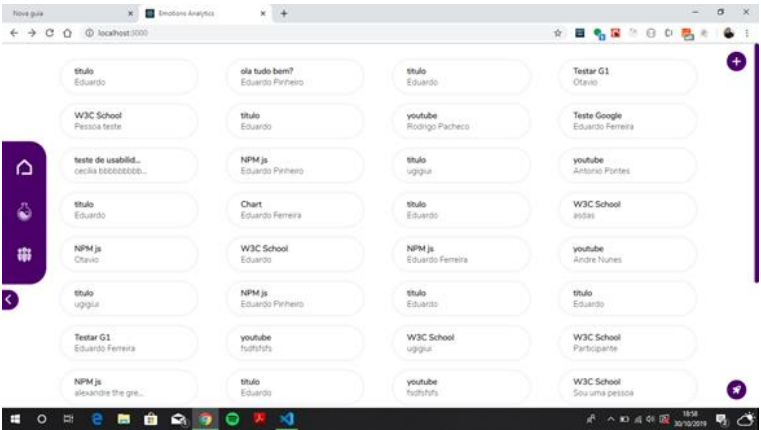
\includegraphics[width=0.7\textwidth]{1}
\end{figure}
\FloatBarrier

\subsection{Tipos de teste}

\subsection{Pessoas}

\begin{figure}[h]
  \caption{Tela de listagem de participantes do sistema}
  \centering
  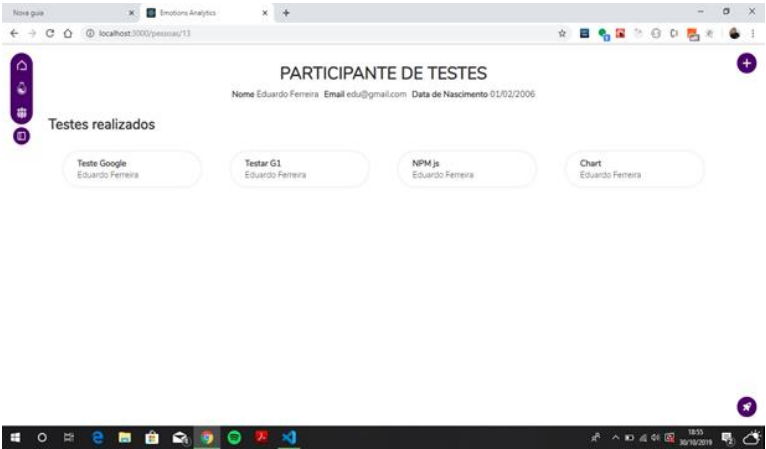
\includegraphics[width=0.7\textwidth]{2}
\end{figure}
\FloatBarrier

\subsection{Cadastro de usuário}

\begin{figure}[h]
  \caption{Tela de cadastro de usuário do sistema}
  \centering
  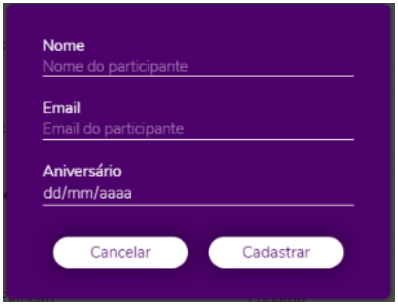
\includegraphics[width=0.7\textwidth]{3}
\end{figure}
\FloatBarrier

\subsection{Cadastro de tipo de teste}

\begin{figure}[h]
  \caption{Tela de cadastro de tipos de teste do sistema}
  \centering
  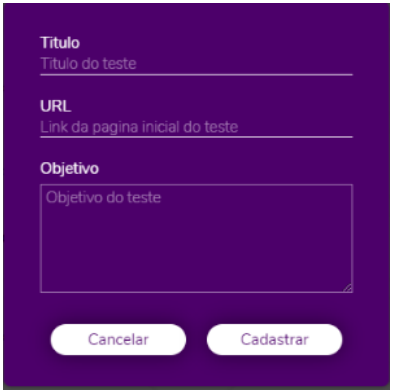
\includegraphics[width=0.7\textwidth]{4}
\end{figure}
\FloatBarrier

\subsection{Inicio do teste}

\begin{figure}[h]
  \caption{Tela de início de testes do sistema}
  \centering
  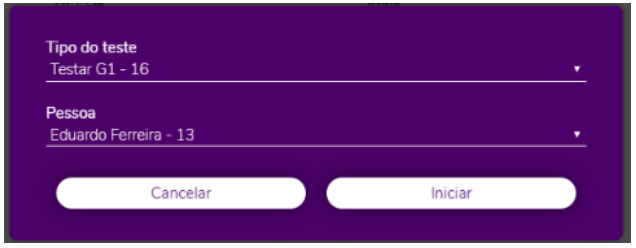
\includegraphics[width=0.7\textwidth]{5}
\end{figure}
\FloatBarrier

\subsection{Relatórios}

\begin{figure}[h]
  \caption{Tela de relatórios do sistema}
  \centering
  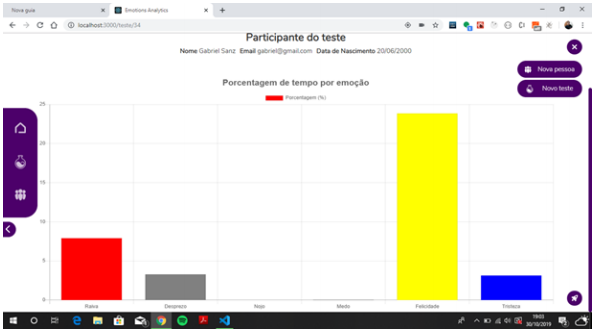
\includegraphics[width=0.7\textwidth]{6}
\end{figure}
\FloatBarrier

\section{Diagramas do sistema}

\subsection{Modelo de Entidade e Relacionamento do sistema \cite{26}}

\begin{figure}[h]
  \caption{Diagrama de Modelo de Entidade e Relacionamento do sistema}
  \centering
  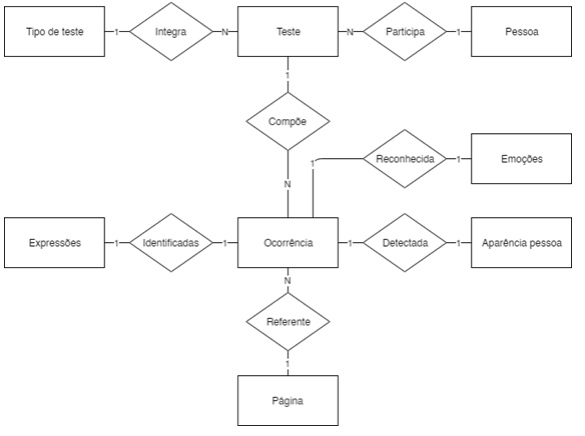
\includegraphics[width=0.7\textwidth]{7}
\end{figure}
\FloatBarrier

\subsection{Diagrama de casos de uso \cite{27}}

\begin{figure}[h]
  \caption{Diagrama de casos de uso do sistema}
  \centering
  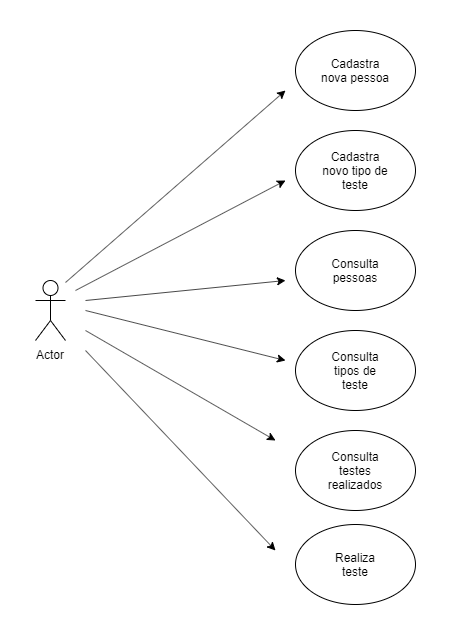
\includegraphics[width=0.7\textwidth]{8}
\end{figure}
\FloatBarrier

\subsection{Diagrama de classes \cite{27}}

\begin{figure}[h]
  \caption{Diagrama de classes do sistema}
  \centering
  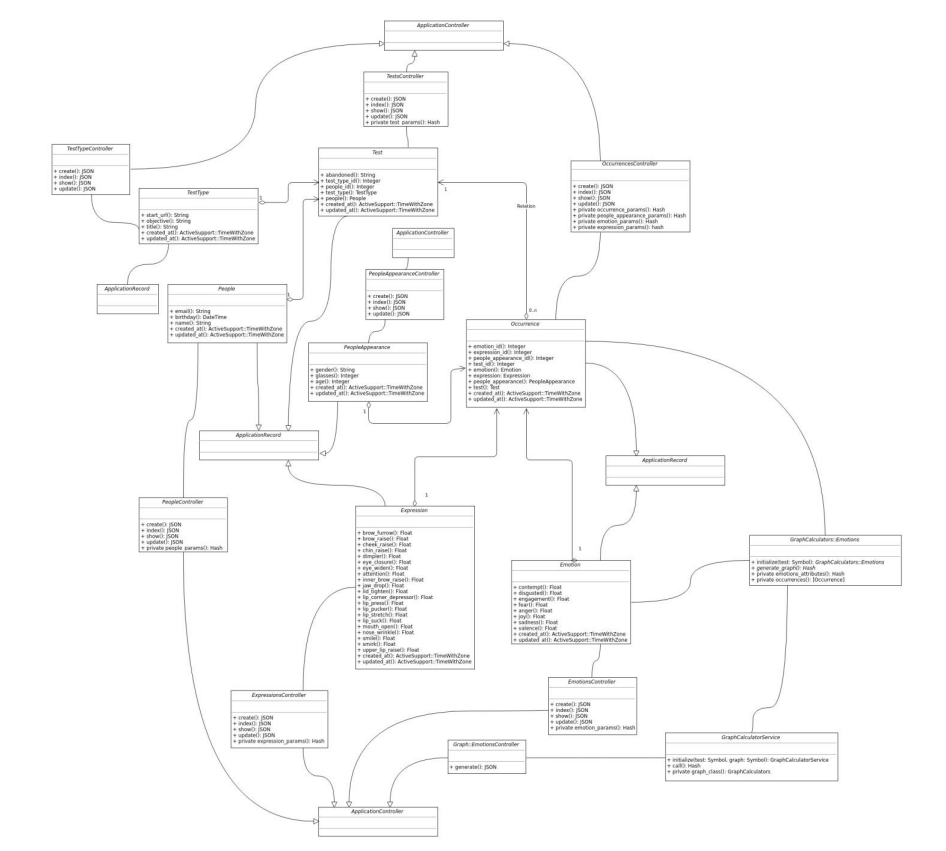
\includegraphics[width=0.7\textwidth]{9}
\end{figure}
\FloatBarrier

\subsection{Diagramas de sequência \cite{28}}

\begin{figure}[h]
  \caption{Diagrama de sequência de criação, edição, leitura e deleção do endpoint TestType do sistema}
  \centering
  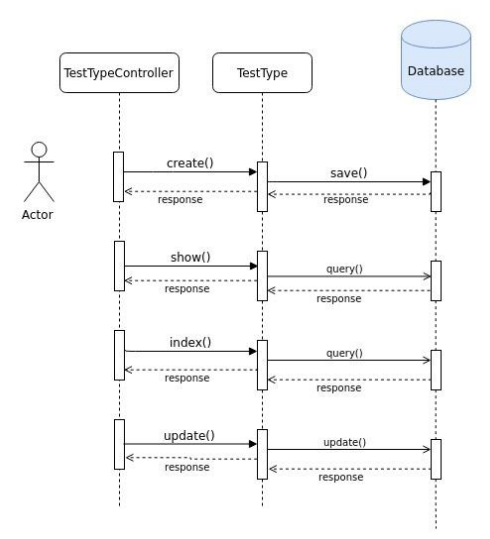
\includegraphics[width=0.7\textwidth]{10}
\end{figure}
\FloatBarrier

\begin{figure}[h]
  \caption{Diagrama de sequência de criação, edição, leitura e deleção do endpoint Tests do sistema}
  \centering
  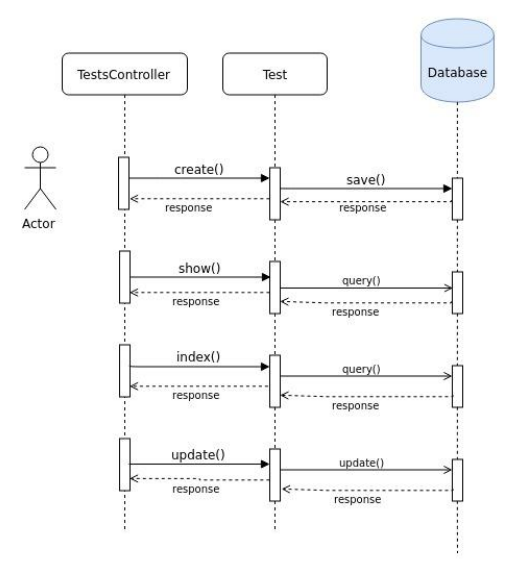
\includegraphics[width=0.7\textwidth]{11}
\end{figure}
\FloatBarrier

\begin{figure}[h]
  \caption{Diagrama de sequência de criação, edição, leitura e deleção do endpoint People do sistema}
  \centering
  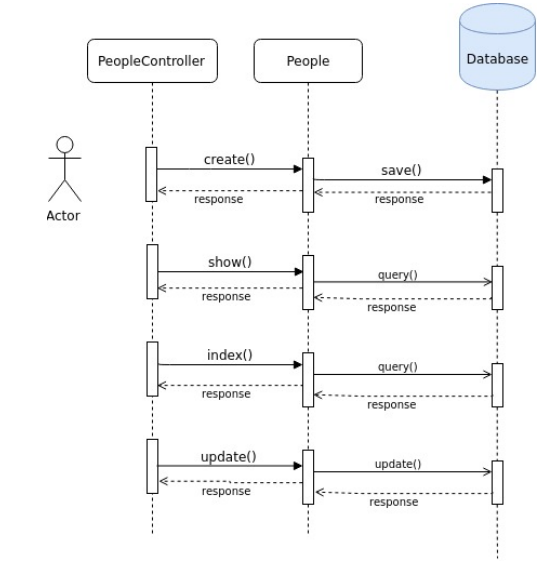
\includegraphics[width=0.7\textwidth]{12}
\end{figure}
\FloatBarrier

\begin{figure}[h]
  \caption{Diagrama de sequência de criação, edição, leitura e deleção do endpoint PeopleAppearence do sistema}
  \centering
  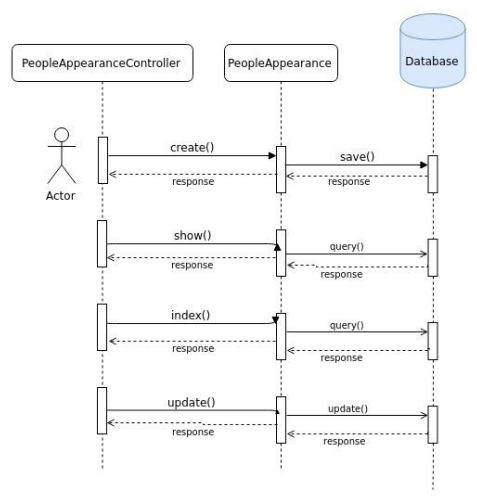
\includegraphics[width=0.7\textwidth]{13}
\end{figure}
\FloatBarrier

\begin{figure}[h]
  \caption{Diagrama de sequência de criação, edição, leitura e deleção do endpoint Expressions do sistema}
  \centering
  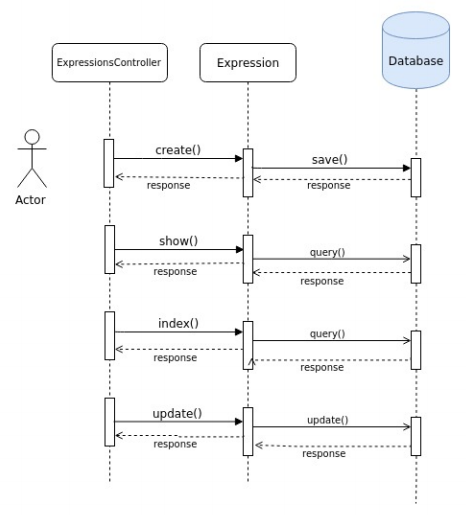
\includegraphics[width=0.7\textwidth]{14}
\end{figure}
\FloatBarrier

\begin{figure}[h]
  \caption{Diagrama de sequência de criação, edição, leitura e deleção do endpoint Emotions do sistema}
  \centering
  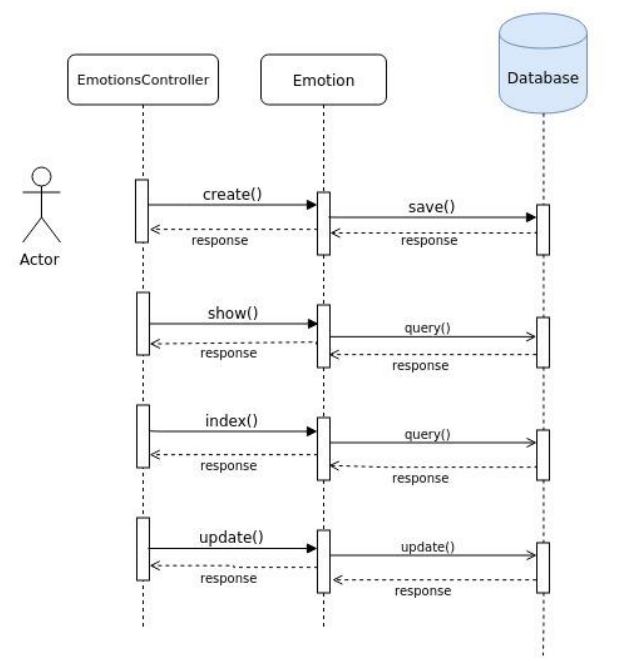
\includegraphics[width=0.7\textwidth]{15}
\end{figure}
\FloatBarrier

\begin{figure}[h]
  \caption{Diagrama de sequência de criação, edição, leitura e deleção do endpoint Occurences do sistema}
  \centering
  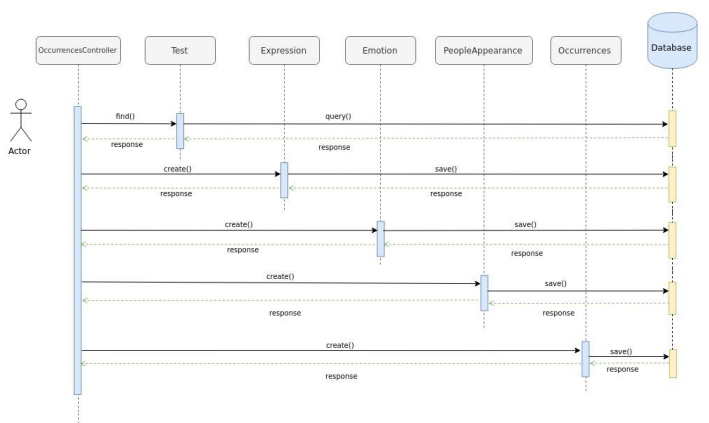
\includegraphics[width=0.7\textwidth]{16}
\end{figure}
\FloatBarrier

\subsection{Diagramas de máquina de estado \cite{30}}

\begin{figure}[h]
  \caption{Diagrama de maquina de estado para cadastro de pessoa no sistema}
  \centering
  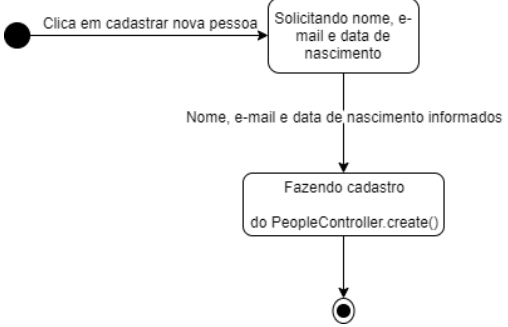
\includegraphics[width=0.7\textwidth]{17}
\end{figure}
\FloatBarrier

\begin{figure}[h]
  \caption{Diagrama de maquina de estado para cadastro de tipo de teste no sistema}
  \centering
  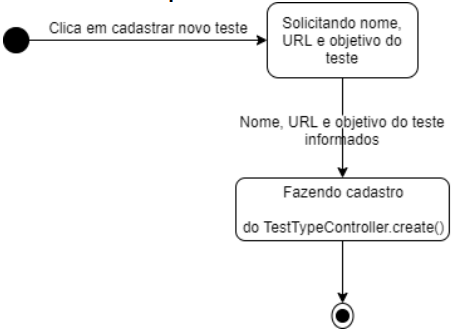
\includegraphics[width=0.7\textwidth]{18}
\end{figure}
\FloatBarrier

\begin{figure}[h]
  \caption{Diagrama de maquina de estado para consulta de pessoa no sistema}
  \centering
  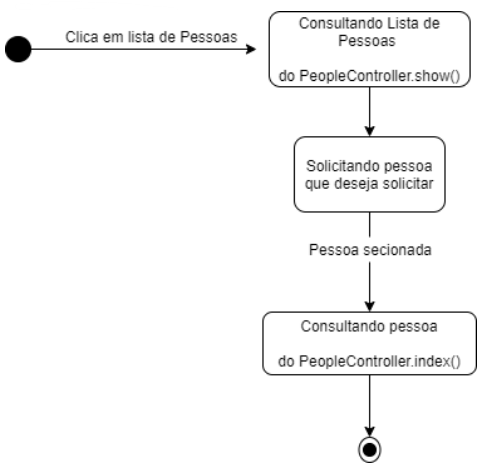
\includegraphics[width=0.7\textwidth]{19}
\end{figure}
\FloatBarrier

\begin{figure}[h]
  \caption{Diagrama de maquina de estado para consulta de tipos de teste no sistema}
  \centering
  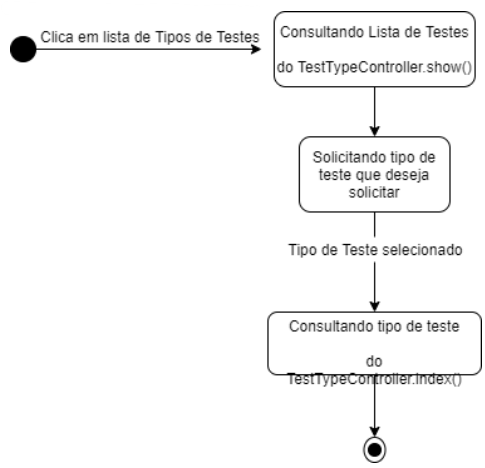
\includegraphics[width=0.7\textwidth]{20}
\end{figure}
\FloatBarrier

\begin{figure}[h]
  \caption{Diagrama de maquina de estado para realizar teste no sistema}
  \centering
  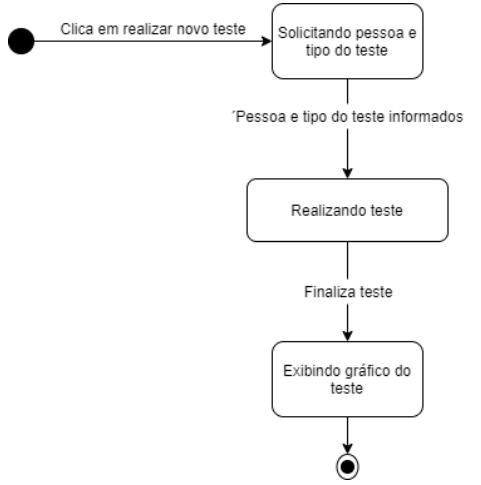
\includegraphics[width=0.7\textwidth]{21}
\end{figure}
\FloatBarrier

\begin{figure}[h]
  \caption{Diagrama de maquina de estado para consulta de teste no sistema}
  \centering
  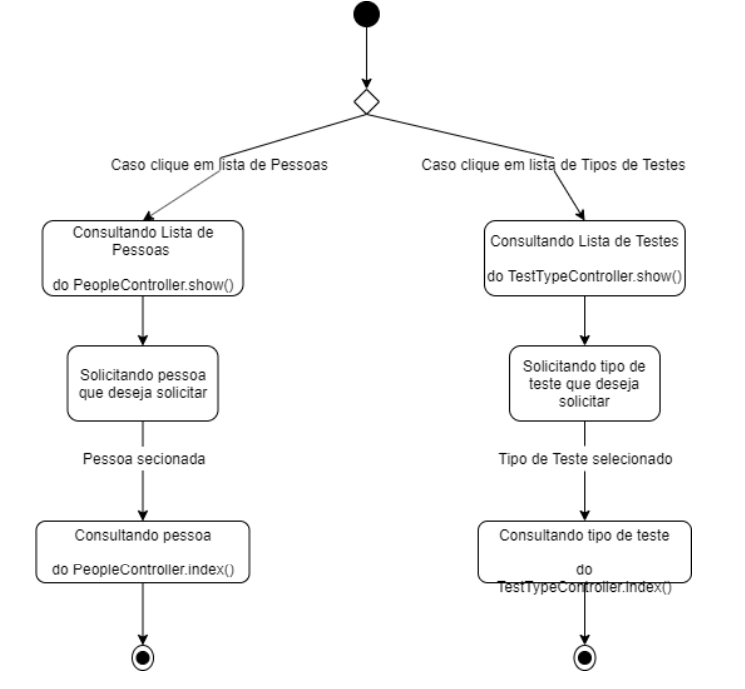
\includegraphics[width=0.7\textwidth]{22}
\end{figure}
\FloatBarrier
